% Copyright 2004 by Till Tantau <tantau@users.sourceforge.net>.
% Copyright 2009 by Barbara Filip <basiaf@fatcat.ftj.agh.edu.pl>
%
% In principle, this file can be redistributed and/or modified under
% the terms of the GNU Public License, version 2.
%
% However, this file is supposed to be a template to be modified
% for your own needs. For this reason, if you use this file as a
% template and not specifically distribute it as part of a another
% package/program, I grant the extra permission to freely copy and
% modify this file as you see fit and even to delete this copyright
% notice. 

\documentclass{beamer}

\mode<presentation>
{
  \usetheme{aghpl}
}

\usepackage[polish]{babel}
% or whatever

%\usepackage[utf8]{inputenc}
% or whatever

\usepackage{times}
\usepackage[T1]{fontenc}
\usepackage{xltxtra}
\usepackage{fontspec}
% Or whatever. Note that the encoding and the font should match. If T1
% does not look nice, try deleting the line with the fontenc.
\usepackage{float}
\usepackage{subcaption}

\title[Krótki Tytuł] % (optional, use only with long paper titles)
{\LARGE Identyfikacja wybranych typów podstruktur w sieciach reprezentujących opinie}

%\subtitle
%{}

\author[Michał Ochman] % (optional, use only with lots of authors)
{Michał Ochman, WFiIS AGH}
% - Give the names in the same order as the appear in the paper.
% - Use the \inst{?} command only if the authors have different
%   affiliation.

\institute[AGH] % (optional, but mostly needed)
{
  opiekun: dr hab. Jarosław Kwapień, IFJ PAN
}
% - Use the \inst command only if there are several affiliations.
% - Keep it simple, no one is interested in your street address.

\date[27 września 2013] % (optional, should be abbreviation of conference name)
{Kraków, 27 września 2013}
% - Either use conference name or its abbreviation.
% - Not really informative to the audience, more for people (including
%   yourself) who are reading the slides online

%\subject{Theoretical Computer Science}
% This is only inserted into the PDF information catalog. Can be left
% out. 



% If you have a file called "university-logo-filename.xxx", where xxx
% is a graphic format that can be processed by latex or pdflatex,
% resp., then you can add a logo as follows:

% \pgfdeclareimage[height=0.5cm]{university-logo}{university-logo-filename}
% \logo{\pgfuseimage{university-logo}}



% Delete this, if you do not want the table of contents to pop up at
% the beginning of each subsection:
% \AtBeginSubsection[]
% {
%  \begin{frame}<beamer>{Outline}
%    \tableofcontents[currentsection,currentsubsection]
%  \end{frame}
% }


% If you wish to uncover everything in a step-wise fashion, uncomment
% the following command: 

%\beamerdefaultoverlayspecification{<+->}


\begin{document}

\begin{frame}
  \titlepage
\end{frame}

\begin{frame}{Plan prezentacji}
  \tableofcontents
  % You might wish to add the option [pausesections]
\end{frame}

\section{Cel pracy}
\begin{frame}{Cel pracy}
  Przedmiotem zainteresowania pracy jest struktura i ewolucja sieci opisujących opinie wybranych grup agentów.
  \pause
  \begin{block}{Źródła problemów:}
    \begin{itemize}
      \item Marketing szeptany (word of mouth).
      \item Promowanie mody (trend setting).
      \item Marketing społecznościowy (community marketing).
    \end{itemize}
  \end{block}
  \pause
  Ze wględu na zaufanie ,,zwykłych'' użytkowników do ,,guru'' istnieje potrzeba wyławiania nieszczerych użytkowników.
\end{frame}

\section{Eksploracja danych}
\begin{frame}{Eksploracja danych}
  Zwykle odkrywanie wiedzy z istniejących baz danych, ale nie tylko.

  Tu, przetwarzanie jednego typu zbioru danych w inny.
  \pause
  \begin{block}{Analiza danych:}
    \begin{itemize}
      \item Asocjacje.
      \item Klasteryzacja.
    \end{itemize}
  \end{block}
\end{frame}

\section{Przetwarzanie języka naturalnego}
\begin{frame}{Przetwarzanie języka naturalnego}
  \begin{block}{Segmentacja i normalizacja}
    Ach, to on! $\to$ [ach; to; on]
  \end{block}
  \pause
  \begin{block}{Klasyfikacja}
    \begin{itemize}
      \item[$\times$] \textit{Stopwords}.
      \item[$\times$] Funktory. 
      \item[\checkmark] Nazwy. 
    \end{itemize}

  \end{block}
  \pause
  \begin{block}{Szukanie rdzenia (lub podstawy słowotwórczej)}
    \begin{itemize}
      \item Usuwanie przyrostków
    \end{itemize}
  \end{block}
\end{frame}

\section{Sieci złożone}
\begin{frame}{Sieci złożone}
  \begin{block}{Grafy:}
    \begin{itemize}
      \item o nieregularnych i nielosowych połączeniach,
      \item o nietrywialnej topologii:
      \begin{itemize}
        \item charakterystyczny rozkład stopni wierzchołków,
        \item wysoki współczynnik klastrowania,
        \item asortatywność.
      \end{itemize}
    \end{itemize}
  \end{block}
  \pause
  \begin{block}{Typy:}
    \begin{itemize}
      \item Sieci społecznościowe
      \item Sieci informacyjne
      \item Sieci biologiczne
    \end{itemize}
  \end{block}
\end{frame}

\section{Małe światy}
\begin{frame}{Małe światy}
  Eksperyment Milgrama -- sześć stopni oddalenia.
  \pause
  \begin{block}{Modele grafów losowych}
    \begin{description}
      \item[Model Erdősa-Rényi'ego] ~\\Prawdopodobieństwo połączenia równe i niezależne od poprzednich połączeń.
      \item[Model Wattsa-Strogatza] ~\\Krótkie średnie długości ścieżek i wysoki współczynnik klastrowania.
      \item[Model Barabásiego–Alberta] ~\\Preferencyjne dołączanie.
    \end{description}
  \end{block}
\end{frame}

\section{Rozkład stopni wierzchołków}
\begin{frame}{Rozkład stopni wierzchołków}
  \begin{figure}[H]
    \centering
    \begin{minipage}[h]{0.49\textwidth}
      \centering
      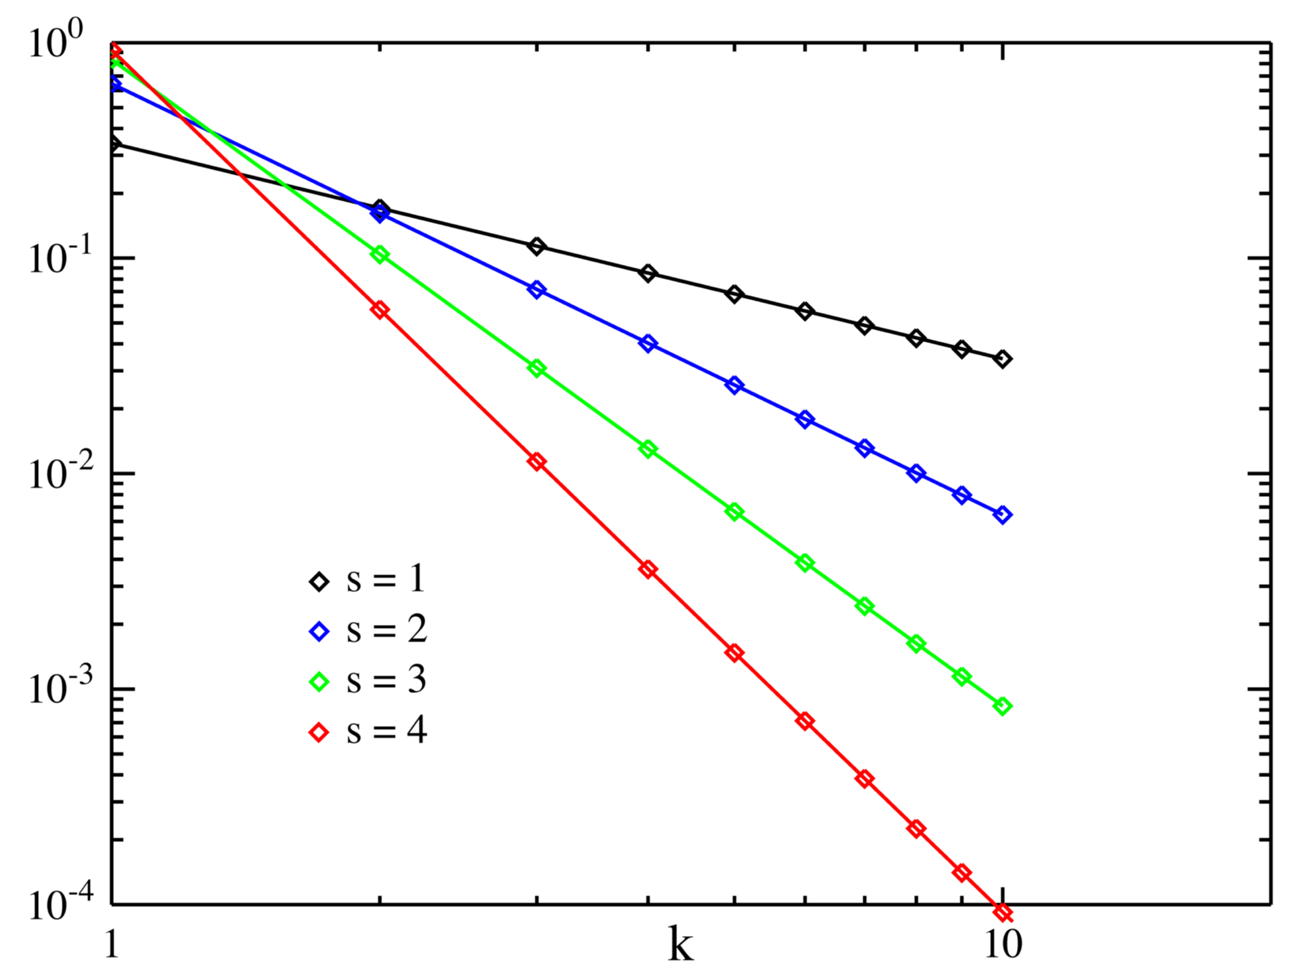
\includegraphics[width=\textwidth]{zipf}
      \caption{Prawo Zipfa}
      \label{fig:path}
    \end{minipage}
    \begin{minipage}[h]{0.49\textwidth}
      Prawo potęgowe:
      \begin{equation}
        P(k) = \frac{n_k}{n} \sim k^{-\gamma} \mbox{,}
      \end{equation}
      gdzie $P(k)$ to prawdopodobieństwo, że dany wierzchołek ma stopień równy $k$, $n$ jest liczbą wierzchołków, a $n_k$ liczbą wierzchołków o stopniu $k$.
    \end{minipage}
  \end{figure}
\end{frame}

\section{Upraszczanie sieci}
\begin{frame}{Upraszczanie sieci}
  Usuwanie krawędzi o mniejszym znaczeniu.
  
  Stosunek współczynnika spójności:
  \begin{equation}
    rk(V, E, E_R) = \frac{C(V, E, E_R)}{C(V, E)} \mbox{,}
  \end{equation}
  gdzie $V$ to zbiór wierzchołków, $E$ to zbiór krawędzi, $E_R$ to zbiór wierzchołków ,,do usunięcia'', a $C(V, E, E_R)$ to spójność grafu po usunięciu z niego krawędzi $E_R$.
  
  \begin{equation}
    0 < rk < 1 \mbox{.}
  \end{equation}

\end{frame}

\section{Szacowanie opinii}
\begin{frame}{Szacowanie opinii}
  Miara szacowanej opinii:
  \begin{equation}
    \frac{1}{1^2} + \frac{1}{2^2} + \frac{1}{3^2} + \frac{1}{4^2} + \ldots = \sum_{n=1}^\infty \frac{1}{n^2} = \frac{\pi^2}{6} \mbox{,}
  \end{equation}
  gdzie $n$ jest odległością opinii od słowa kluczowego.

  Przedział wartości miary:
  \begin{equation}
    -\frac{\pi^2}{3} \leq e_o \leq \frac{\pi^2}{3} \mbox{,}
  \end{equation}
  wynika z możliwości położenia opinii zarówno przed jak i po słowie kluczowym.

\end{frame}

\section{Collaborative similarity}
\begin{frame}{Collaborative similarity}
  \begin{figure}[H]
    \centering
    \begin{minipage}[h]{0.4\textwidth}
      \centering
      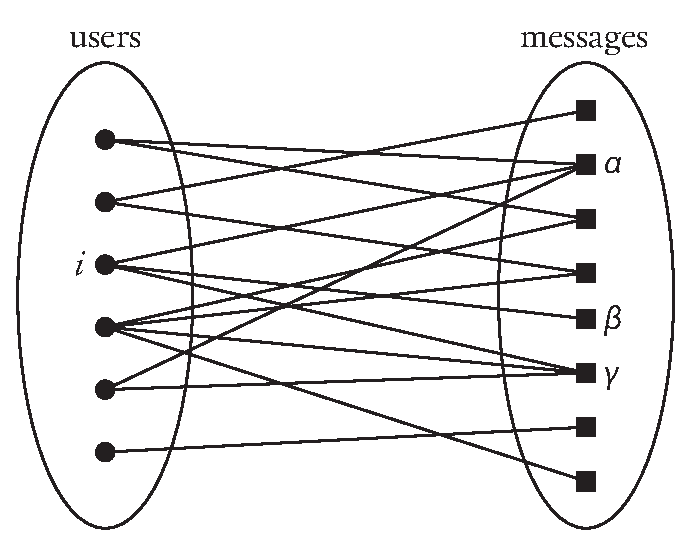
\includegraphics[width=\textwidth]{cs_network}
      \caption{Sieć dwudzielna}
      \label{fig:path}
    \end{minipage}
    \begin{minipage}[h]{0.58\textwidth}
      \begin{equation}
        d_{nn}(i) = \frac{d_\alpha + d_\beta + d_\gamma}{3} = \frac{7}{3} \mbox{.}
      \end{equation}
      \begin{equation}
        s_{\beta\gamma} = \frac{\Gamma_\beta \cap \Gamma_\gamma}{\Gamma_\beta \cup \Gamma_\gamma} = \frac{1}{3} \mbox{.}
      \end{equation}
      \begin{equation}
        C_u(i) = \frac{1}{k_i(k_i-1)} \sum_{\alpha\neq\beta} s_{\alpha\beta}\mbox{.}
      \end{equation}
    \end{minipage}
  \end{figure}
\end{frame}

\section{Motywy}
\begin{frame}{Motywy}
  \begin{figure}[h]
    \centering
    \begin{subfigure}[b]{0.3\textwidth}
      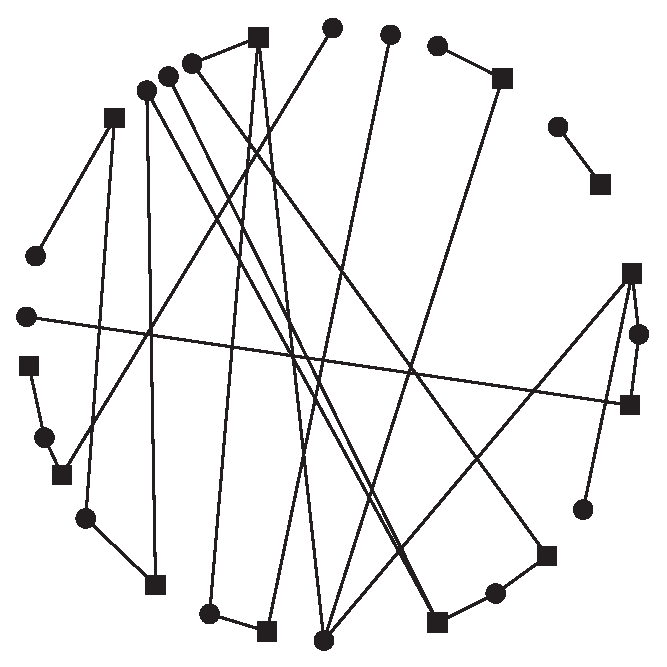
\includegraphics[width=\textwidth]{cs_motif_1}
      \caption{Krok 1.}
    \end{subfigure}
    \begin{subfigure}[b]{0.3\textwidth}
      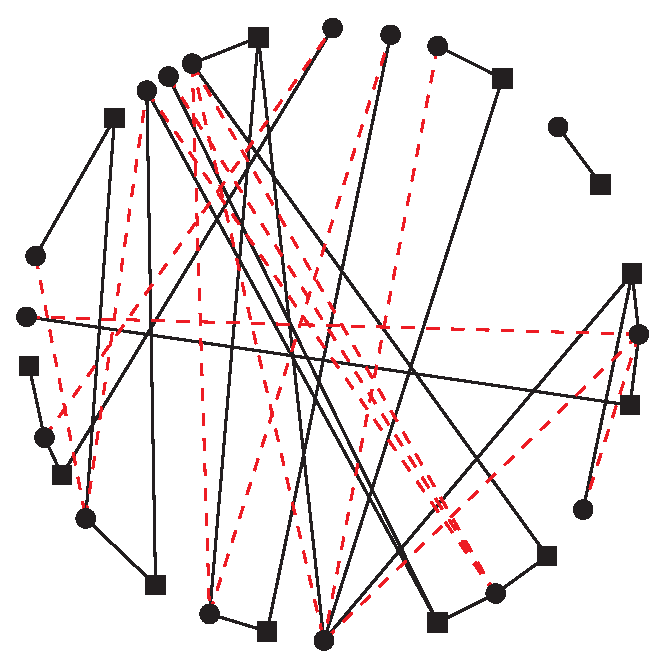
\includegraphics[width=\textwidth]{cs_motif_2}
      \caption{Krok 2.}
    \end{subfigure}
    \begin{subfigure}[b]{0.3\textwidth}
      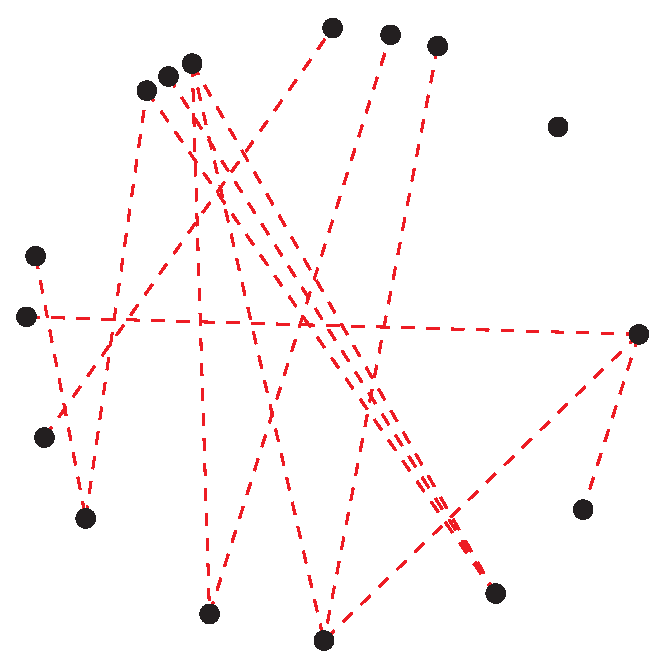
\includegraphics[width=\textwidth]{cs_motif_3}
      \caption{Krok 3.}
    \end{subfigure}
    \caption{Wyszukiwanie motywów.}
  \end{figure}
  Koła to użytkownicy, a kwadraty to słowa kluczowe. Linie ciągłe reprezentują słowa użyte przez użytkowników, a przerywane uzyskane połączenia między użytkownikami.
\end{frame}

\section*{Podsumowanie}
\begin{frame}{Podsumowanie}
  \begin{block}{Efekty:}
    \begin{itemize}
      \item Nie udało się znaleźć ,,nieszczerych'' użytkowników.
      \item Zaproponowano miarę szacowania opinii oraz zaprezentowano sposób jej użycia.
    \end{itemize}
  \end{block}
  \pause
  \begin{block}{Co dalej?}
    \begin{itemize}
      \item System rekomendujący na podstawie zmian w opiniach.
      \item Oszacowanie ,,idealnego'' czasu na prowadzenie akcji marketingowej.
    \end{itemize}
  \end{block}
\end{frame}

\section*{Koniec}
\begin{frame}{Koniec}
\Huge Dziękuję za uwagę.
\end{frame}

\end{document}